\documentclass{article}

% if you need to pass options to natbib, use, e.g.:
%     \PassOptionsToPackage{numbers, compress}{natbib}
% before loading neurips_2019

% ready for submission
% \usepackage{neurips_2019}

% to compile a preprint version, e.g., for submission to arXiv, add add the
% [preprint] option:
%     \usepackage[preprint]{neurips_2019}

% to compile a camera-ready version, add the [final] option, e.g.:
\usepackage[final]{neurips_2019}

% to avoid loading the natbib package, add option nonatbib:
%     \usepackage[nonatbib]{neurips_2019}

\usepackage[utf8]{inputenc} % allow utf-8 input
\usepackage[T1]{fontenc}    % use 8-bit T1 fonts
\usepackage{hyperref}       % hyperlinks
\usepackage{url}            % simple URL typesetting
\usepackage{booktabs}       % professional-quality tables
\usepackage{amsfonts}       % blackboard math symbols
\usepackage{nicefrac}       % compact symbols for 1/2, etc.
\usepackage{microtype}      % microtypography
\usepackage{amsfonts}
\usepackage{amsmath}
\usepackage{graphicx}
\graphicspath{ {./images/} }

\title{Univariate Time Series Forecasting using ES-RNN and N-BEATS}

% The \author macro works with any number of authors. There are two commands
% used to separate the names and addresses of multiple authors: \And and \AND.
%
% Using \And between authors leaves it to LaTeX to determine where to break the
% lines. Using \AND forces a line break at that point. So, if LaTeX puts 3 of 4
% authors names on the first line, and the last on the second line, try using
% \AND instead of \And before the third author name.
\author{%
  Yves Greatti \\
  New York University\\
  \texttt{yves.greatti@nyu.edu} \\
  % examples of more authors
   \And
    Zian Chen \\
    New York University\\
    \texttt{zian.chen@nyu.edu} \\
    \And 
   Sunjoo Park\\
    New York University\\
    \texttt{sunjoo.park@nyu.edu}
}
\begin{document}

\maketitle

\begin{abstract}
  In this work, we seek to replicate and improve the results reached by two neural networks: \textbf{ES-RNN} and \textbf{N-BEATS} on the M4 dataset competition.
  We also run different experimentations to compare the performances of these two deep learning techniques to a more classical statistical approach like Gaussian Process ($\mathcal{GP}$).
  We demonstrate that although Gaussian processes could be powerful for sampling tasks and simpler to configure, these neural networks outperform it for forecasting. Neural networks could have an overhead in term of the number of hyper-parameters to tune, but when using batching they scale up very easily and generalize well to a large number of time series (100K for M4). We are thus, pretty confident that, the two neural networks could handle with the appropriate setting of hyper-parameters, other univariate time series beyond the M4 dataset.  
  
 \end{abstract}

\section{Introduction}

\paragraph{Summary} The dataset is provided by the M4 competition organized by the International Institute of Forecasters. These competitions also know as the "Madrakis competitions", have been happening since 1982, roughly every 10 years with an increasing number of time series to forecast starting from 1001in 1982  to 100,000 in 2018, the M4 competition. They attract people from academia as well practitioners, the last winner being Slawek Smyl, from Uber Technologies. The model used by Smyl is a hybrid approach combining Holts-Winter smoothing techniques with a recurrent neural network (RNN). Boris Oreshkin et Al. want to challenge the conclusion that, mixed techniques are the future by proposing a pure DL model with interpretable outputs: \textbf{N-Beats}, which they claim outperforms \textbf{ES-RNN}, Smyl's model. N-Beats could be a very deep DL model and it is important for their authors that, in addition to hight accuracy, N-Beats has interpretable outputs which can match established statistical models such as ETS and ARIMA, which are robust, efficient, and automatic. 

\section{ES-RNN}
\label{ESRNN}

\subsection{Model Description}

ES-RNN algorithm consists in two major layers: a preprocessing layer which uses Holt-Winter smoothing technic to extract trend and seasonality parameters and a dilated RNN network.
The Holt-Winter parameters are part of the back-propagation and are tuned as the network learns the characteristics of the time series. The ES-RNN model uses a modified version of the Holt-Winters formula,
in which there is no local linear level coefficient, and level and seasonality terms are scaled instead of subtracted. 
The linear forecast is replaced by an RNN, which has for input the normalized and de-seasonalized prior observations. 


\begin{align*}
	l_t 	&= \alpha \frac{y_t} {s_{t-m}} + (1-\alpha) l_{t-1} \\
	s_t 	&= \beta \frac{y_t}{l_{t-1}} + (1-\beta) s_{t-m} \\
	\hat{y}_{\textbf{win}}		&= \textbf{ES-RNN}(\frac{y_{ti}}{s_{ti} l_{ti}}) \\
	y_{\textbf{truth}}		&= (\frac{y_{to}}{s_{to} l_{to}}) 
\end{align*}
where $l$ is a state variable, $s$ is a seasonality coefficient, $\alpha$ and $\beta$ are network parameters, $m$ is the periodicity of the data.

To model long-term dependencies in time series, ES-RNN uses dilated RNNs which allow to stack RNN cells by having skip connections between RNN cells . 
The dilation parameters  are given in table \autoref{tab:dilations}  DRNN cells can be vanilla RNN, LSTM, GRU,  GRU cells provided the higher accuracy.

\begin{table}[!ht]
	\centering
	\begin{tabular}{ll} \toprule
		\textbf{Time Series} & \textbf{Dilations} \\ 
		\midrule
		Quarterly  & (1, 2), (4, 8)	\\
		\midrule
		Monthly 	& (1, 3), (6, 12)	\\
		\midrule
		Daily 	& (1, 7), (14, 28)	\\
		\midrule		
		Yearly 	& (1, 2), (2, 6) 	\\
		\midrule		
		Weekly 	& (1, 14), (14, 28)	\\
		\midrule		
		Hourly 	& (1, 24), (24, 48)	\\
		%\bottomrule
	\end{tabular}
	\label{tab:dilations}
	\caption{ES-RNN dilation parameters}
\end{table}


 \subsection{Data Preparation}
 The M4 time series have different length, to allow vectorization and to take advantage of the GPUs, they are chopped using a predetermined cut off value.
 To the exception of the daily time series, for which the cut-off value is 200, 72 is used as the default value (\autoref{tab:cutoff}.
 
 \begin{table}[!ht]
	\centering
	\begin{tabular}{llllllll} 
	\toprule
		& \multicolumn{6}{c} {\textbf{Filtering rates (in \%)}} \\
			& \textbf{Hourly} & \textbf{Daily} & \textbf{Weekly} & \textbf{Monthly} & \textbf{Quarterly}   & \textbf{Yearly} \\
		\midrule
		 	& 6.93 	& 6.93  & 18.11 & 26.83 &  45.42 & 60.61 \\
		\bottomrule
	\end{tabular}
	\label{tab:cutoff}
	\caption{Percentage of time series eliminated by the cut-off value}
\end{table}


 The batch size is by default 1024, we noticed that it affects the overall performance of the network, depending the time series frequency,
 too small the validation loss may jump up and down,  and  in some cases the larger the batch size, the better.
 
 For an hourly frequency, the effect of the batch size is given in table  \autoref{tab:batchsize} .
 \begin{table}[!ht]
	\centering
	\begin{tabular}{llllllll} \toprule
			& \multicolumn{6}{c} {\textbf{sMAPE per category}} \\
		\textbf{Batch size} & \textbf{Demographic} & \textbf{Finance} & \textbf{Industry} & \textbf{Macro} & \textbf{Micro} & \textbf{Other} & \textbf{Total}  \\ \midrule
		512 & 6.32 & 3.34 & 3.95 & 2.52 & 2.43 & 3.08 & 3.02 \\
		\midrule
		1024 & 6.20 & 3.27 & 3.9 & 2.52 & 2.37 & 3.07 & 2.97 \\
		\midrule
		2048 & 6.26 & 3.32 & 3.92 & 2.49 & 2.42 & 3.1 & 3.01 \\
		 \bottomrule
	\end{tabular}
	\label{tab:batchsize}
	\caption{ES-RNN batch size statistics}
\end{table}
 
 Each time series is split into two windows: a backcast and forecast window.  Observations in each window are normalized and de-seasonalized using the coefficients of the exponential smoothing.
 In addition, a one-hot representation of the time series category is added to the input window.
 
 \begin{center}
	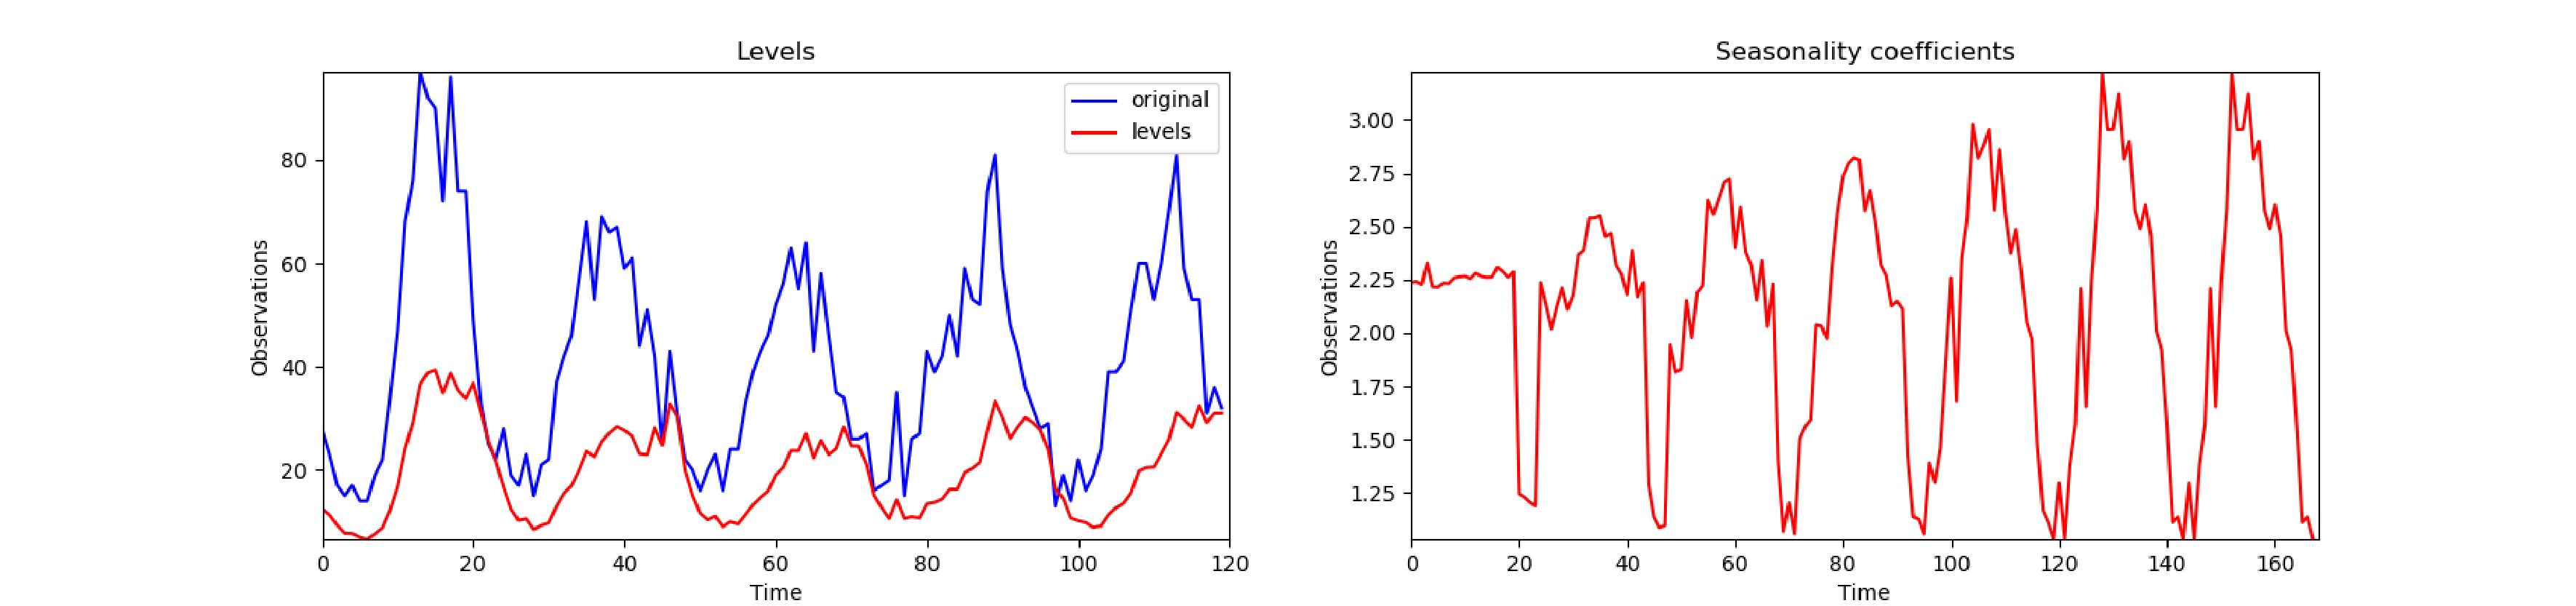
\includegraphics{H344_levels_seasonalities.pdf} 
%	\includegraphics[scale=1,bb=0 0 30 30][width=0.5\linewidth]{H344_levels_seasonalities.png} 
\end{center}

\section{General formatting instructions}
\label{gen_inst}

The text must be confined within a rectangle 5.5~inches (33~picas) wide and
9~inches (54~picas) long. The left margin is 1.5~inch (9~picas).  Use 10~point
type with a vertical spacing (leading) of 11~points.  Times New Roman is the
preferred typeface throughout, and will be selected for you by default.
Paragraphs are separated by \nicefrac{1}{2}~line space (5.5 points), with no
indentation.

The paper title should be 17~point, initial caps/lower case, bold, centered
between two horizontal rules. The top rule should be 4~points thick and the
bottom rule should be 1~point thick. Allow \nicefrac{1}{4}~inch space above and
below the title to rules. All pages should start at 1~inch (6~picas) from the
top of the page.

For the final version, authors' names are set in boldface, and each name is
centered above the corresponding address. The lead author's name is to be listed
first (left-most), and the co-authors' names (if different address) are set to
follow. If there is only one co-author, list both author and co-author side by
side.

Please pay special attention to the instructions in Section \ref{others}
regarding figures, tables, acknowledgments, and references.

\section{Headings: first level}
\label{headings}

All headings should be lower case (except for first word and proper nouns),
flush left, and bold.

First-level headings should be in 12-point type.

\subsection{Headings: second level}

Second-level headings should be in 10-point type.

\subsubsection{Headings: third level}

Third-level headings should be in 10-point type.

\paragraph{Paragraphs}

There is also a \verb+\paragraph+ command available, which sets the heading in
bold, flush left, and inline with the text, with the heading followed by 1\,em
of space.

\section{Citations, figures, tables, references}
\label{others}

These instructions apply to everyone.

\subsection{Citations within the text}

The \verb+natbib+ package will be loaded for you by default.  Citations may be
author/year or numeric, as long as you maintain internal consistency.  As to the
format of the references themselves, any style is acceptable as long as it is
used consistently.

The documentation for \verb+natbib+ may be found at
\begin{center}
  \url{http://mirrors.ctan.org/macros/latex/contrib/natbib/natnotes.pdf}
\end{center}
Of note is the command \verb+\citet+, which produces citations appropriate for
use in inline text.  For example,
\begin{verbatim}
   \citet{hasselmo} investigated\dots
\end{verbatim}
produces
\begin{quote}
  Hasselmo, et al.\ (1995) investigated\dots
\end{quote}

If you wish to load the \verb+natbib+ package with options, you may add the
following before loading the \verb+neurips_2019+ package:
\begin{verbatim}
   \PassOptionsToPackage{options}{natbib}
\end{verbatim}

If \verb+natbib+ clashes with another package you load, you can add the optional
argument \verb+nonatbib+ when loading the style file:
\begin{verbatim}
   \usepackage[nonatbib]{neurips_2019}
\end{verbatim}

As submission is double blind, refer to your own published work in the third
person. That is, use ``In the previous work of Jones et al.\ [4],'' not ``In our
previous work [4].'' If you cite your other papers that are not widely available
(e.g., a journal paper under review), use anonymous author names in the
citation, e.g., an author of the form ``A.\ Anonymous.''

\subsection{Footnotes}

Footnotes should be used sparingly.  If you do require a footnote, indicate
footnotes with a number\footnote{Sample of the first footnote.} in the
text. Place the footnotes at the bottom of the page on which they appear.
Precede the footnote with a horizontal rule of 2~inches (12~picas).

Note that footnotes are properly typeset \emph{after} punctuation
marks.\footnote{As in this example.}

\subsection{Figures}

\begin{figure}
  \centering
  \fbox{\rule[-.5cm]{0cm}{4cm} \rule[-.5cm]{4cm}{0cm}}
  \caption{Sample figure caption.}
\end{figure}

All artwork must be neat, clean, and legible. Lines should be dark enough for
purposes of reproduction. The figure number and caption always appear after the
figure. Place one line space before the figure caption and one line space after
the figure. The figure caption should be lower case (except for first word and
proper nouns); figures are numbered consecutively.

You may use color figures.  However, it is best for the figure captions and the
paper body to be legible if the paper is printed in either black/white or in
color.

\subsection{Tables}

All tables must be centered, neat, clean and legible.  The table number and
title always appear before the table.  See Table~\ref{sample-table}.

Place one line space before the table title, one line space after the
table title, and one line space after the table. The table title must
be lower case (except for first word and proper nouns); tables are
numbered consecutively.

Note that publication-quality tables \emph{do not contain vertical rules.} We
strongly suggest the use of the \verb+booktabs+ package, which allows for
typesetting high-quality, professional tables:
\begin{center}
  \url{https://www.ctan.org/pkg/booktabs}
\end{center}
This package was used to typeset Table~\ref{sample-table}.

\begin{table}
  \caption{Sample table title}
  \label{sample-table}
  \centering
  \begin{tabular}{lll}
    \toprule
    \multicolumn{2}{c}{Part}                   \\
    \cmidrule(r){1-2}
    Name     & Description     & Size ($\mu$m) \\
    \midrule
    Dendrite & Input terminal  & $\sim$100     \\
    Axon     & Output terminal & $\sim$10      \\
    Soma     & Cell body       & up to $10^6$  \\
    \bottomrule
  \end{tabular}
\end{table}

\section{Final instructions}

Do not change any aspects of the formatting parameters in the style files.  In
particular, do not modify the width or length of the rectangle the text should
fit into, and do not change font sizes (except perhaps in the
\textbf{References} section; see below). Please note that pages should be
numbered.

\section{Preparing PDF files}

Please prepare submission files with paper size ``US Letter,'' and not, for
example, ``A4.''

Fonts were the main cause of problems in the past years. Your PDF file must only
contain Type 1 or Embedded TrueType fonts. Here are a few instructions to
achieve this.

\begin{itemize}

\item You should directly generate PDF files using \verb+pdflatex+.

\item You can check which fonts a PDF files uses.  In Acrobat Reader, select the
  menu Files$>$Document Properties$>$Fonts and select Show All Fonts. You can
  also use the program \verb+pdffonts+ which comes with \verb+xpdf+ and is
  available out-of-the-box on most Linux machines.

\item The IEEE has recommendations for generating PDF files whose fonts are also
  acceptable for NeurIPS. Please see
  \url{http://www.emfield.org/icuwb2010/downloads/IEEE-PDF-SpecV32.pdf}

\item \verb+xfig+ "patterned" shapes are implemented with bitmap fonts.  Use
  "solid" shapes instead.

\item The \verb+\bbold+ package almost always uses bitmap fonts.  You should use
  the equivalent AMS Fonts:
\begin{verbatim}
   \usepackage{amsfonts}
\end{verbatim}
followed by, e.g., \verb+\mathbb{R}+, \verb+\mathbb{N}+, or \verb+\mathbb{C}+
for $\mathbb{R}$, $\mathbb{N}$ or $\mathbb{C}$.  You can also use the following
workaround for reals, natural and complex:
\begin{verbatim}
   \newcommand{\RR}{I\!\!R} %real numbers
   \newcommand{\Nat}{I\!\!N} %natural numbers
   \newcommand{\CC}{I\!\!\!\!C} %complex numbers
\end{verbatim}
Note that \verb+amsfonts+ is automatically loaded by the \verb+amssymb+ package.

\end{itemize}

If your file contains type 3 fonts or non embedded TrueType fonts, we will ask
you to fix it.

\subsection{Margins in \LaTeX{}}

Most of the margin problems come from figures positioned by hand using
\verb+\special+ or other commands. We suggest using the command
\verb+\includegraphics+ from the \verb+graphicx+ package. Always specify the
figure width as a multiple of the line width as in the example below:
\begin{verbatim}
   \usepackage[pdftex]{graphicx} ...
   \includegraphics[width=0.8\linewidth]{myfile.pdf}
\end{verbatim}
See Section 4.4 in the graphics bundle documentation
(\url{http://mirrors.ctan.org/macros/latex/required/graphics/grfguide.pdf})

A number of width problems arise when \LaTeX{} cannot properly hyphenate a
line. Please give LaTeX hyphenation hints using the \verb+\-+ command when
necessary.

\subsubsection*{Acknowledgments}

Use unnumbered third level headings for the acknowledgments. All acknowledgments
go at the end of the paper. Do not include acknowledgments in the anonymized
submission, only in the final paper.

\section*{References}

References follow the acknowledgments. Use unnumbered first-level heading for
the references. Any choice of citation style is acceptable as long as you are
consistent. It is permissible to reduce the font size to \verb+small+ (9 point)
when listing the references. {\bf Remember that you can use more than eight
  pages as long as the additional pages contain \emph{only} cited references.}
\medskip

\small

[1] Alexander, J.A.\ \& Mozer, M.C.\ (1995) Template-based algorithms for
connectionist rule extraction. In G.\ Tesauro, D.S.\ Touretzky and T.K.\ Leen
(eds.), {\it Advances in Neural Information Processing Systems 7},
pp.\ 609--616. Cambridge, MA: MIT Press.

[2] Bower, J.M.\ \& Beeman, D.\ (1995) {\it The Book of GENESIS: Exploring
  Realistic Neural Models with the GEneral NEural SImulation System.}  New York:
TELOS/Springer--Verlag.

[3] Hasselmo, M.E., Schnell, E.\ \& Barkai, E.\ (1995) Dynamics of learning and
recall at excitatory recurrent synapses and cholinergic modulation in rat
hippocampal region CA3. {\it Journal of Neuroscience} {\bf 15}(7):5249-5262.

\end{document}
